
\begin{itemize}
    \item \textbf{Conveyor Belt Layer}
    \begin{itemize}
        \item ON/OFF Controller
    \end{itemize}

    \item \textbf{Safety Sensor Layer}
    \begin{itemize}
        \item Computer Vision
        \item UR20 Arm Speed Controller
    \end{itemize}

    \item \textbf{UR20 Robot Arm Layer}
    \begin{itemize}
        \item Vacuum Gripper
        \item Grab Release Control
        \item Movement
    \end{itemize}

    \item \textbf{PLC Layer}
    \begin{itemize}
        \item Input Function
        \item Box Offset Algorithm
        \item Position Algorithm
    \end{itemize}
\end{itemize}
\begin{figure}[h!]
	\centering
 	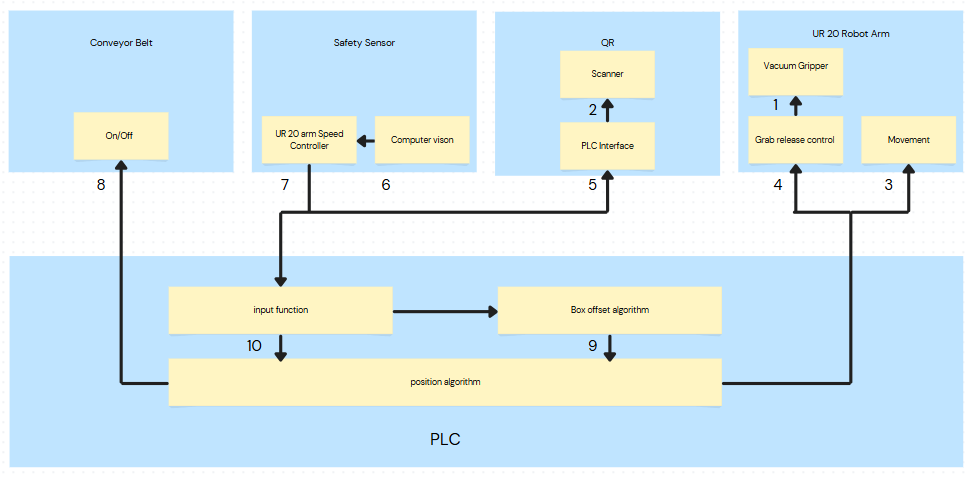
\includegraphics[width=\textwidth]{images/data_flow}
 \caption{UR20 Data flow diagram}
\end{figure}